\documentclass[twocolumn,a4j]{jsarticle}
\setlength{\topmargin}{-20.4cm}
\setlength{\oddsidemargin}{-10.4mm}
\setlength{\evensidemargin}{-10.4mm}
\setlength{\textwidth}{18cm}
\setlength{\textheight}{26cm}

\usepackage[top=15truemm,bottom=25truemm,left=20truemm,right=20truemm]{geometry}
\usepackage[latin1]{inputenc}
\usepackage{amsmath}
\usepackage{amsfonts}
\usepackage{amssymb}
\usepackage[dvipdfmx]{graphicx}
\usepackage[dvipdfmx]{color}
\usepackage{listings}
\usepackage{listings,jvlisting}
\usepackage{geometry}
\usepackage{framed}
\usepackage{color}
\usepackage[dvipdfmx]{hyperref}
\usepackage{ascmac}
\usepackage{enumerate}
\usepackage{tabularx}
\usepackage{cancel}
\usepackage{scalefnt}

\renewcommand{\figurename}{Fig.}
\renewcommand{\tablename}{Table }

\lstset{
basicstyle={\ttfamily},
identifierstyle={\small},
commentstyle={\smallitshape},
keywordstyle={\small\bfseries},
ndkeywordstyle={\small},
stringstyle={\small\ttfamily},
frame={tb},
breaklines=true,
columns=[l]{fullflexible},
xrightmargin=0zw,
xleftmargin=3zw,
numberstyle={\scriptsize},
stepnumber=1,
numbersep=1zw,
lineskip=-0.5ex
}

\makeatletter
\def\@maketitle
{
\begin{center}
{\LARGE \@title \par}
\end{center}
\begin{flushright}
{\large \@date}\\
{\large{京都工芸繊維大学 工芸科学部 機械工学課程}}\\
{\large \@author}
\end{flushright}
\par\vskip 1.5em
}
\makeatother

\setcounter{tocdepth}{3}

\author{来代 勝胤}
\title{令和3年度 11月度 報告書}
\date{2021/11/30}

\begin{document}
\columnseprule=0.1mm

\maketitle
\section*{報告内容}
\begin{enumerate}[1.]
    \item 校正実験の再実施
    \item オフセット値の考慮
    \item 卒業研究について
    \item 実験装置の製作
    \item 実験結果
    \item 今月の進捗と12月の予定
\end{enumerate}

\section{校正実験の再実施}
ロードセルを用いた校正実験において,
微小な作用力が加わる範囲でロードセルの出力電圧に
出力電圧の非線形領域が存在する懸念があったため,
微小な作用力による出力電圧の変化を調べるための校正実験を行った.\\

\subsection{校正実験(1) ロードセルと荷重の関係}
以下のFig.1に2021年6月に行ったロードセルの出力電圧と荷重に関する校正実験の結果を示す.

\begin{figure}[htbp]
    \footnotesize
    \begin{center}
        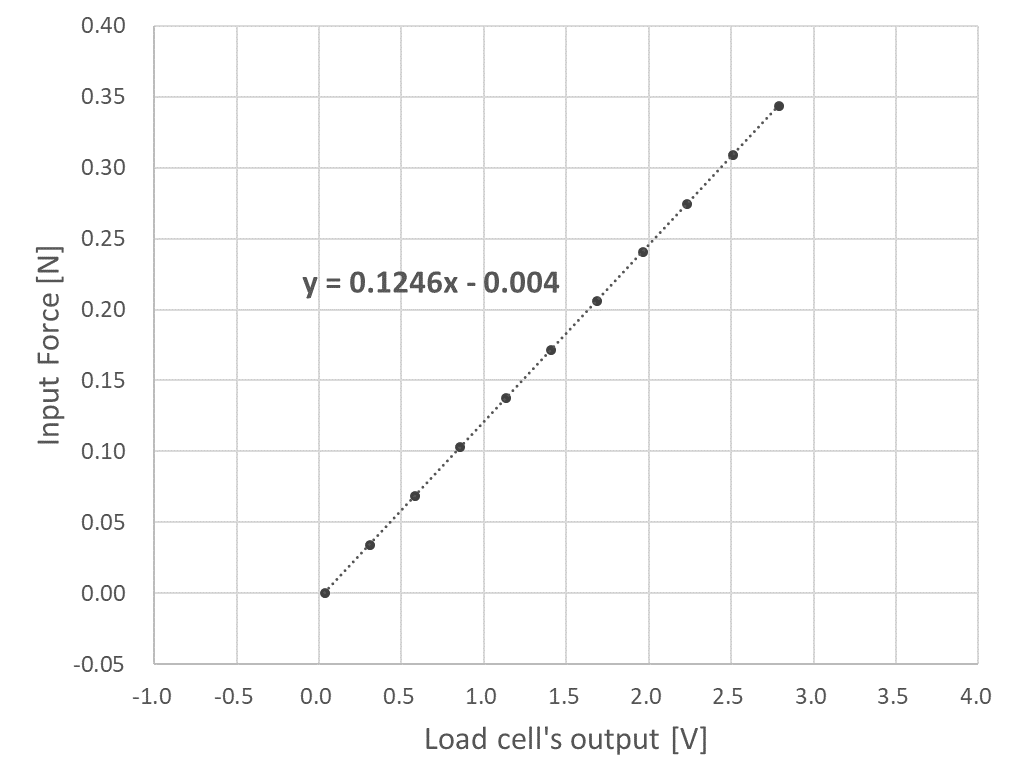
\includegraphics[width=68mm]{../images/calibration_1.png}
        \caption{Previous data of load cell - input force}
    \end{center}
\end{figure}

\newpage

\subsection{校正実験(2) ロードセルとひずみセンサの関係}
以下のFig.2,Fig.3に2021年6月に行った
ロードセルの出力電圧とひずみセンサの出力電圧に関する校正実験の結果を示す.

\begin{figure}[htbp]
    \footnotesize
    \begin{center}
        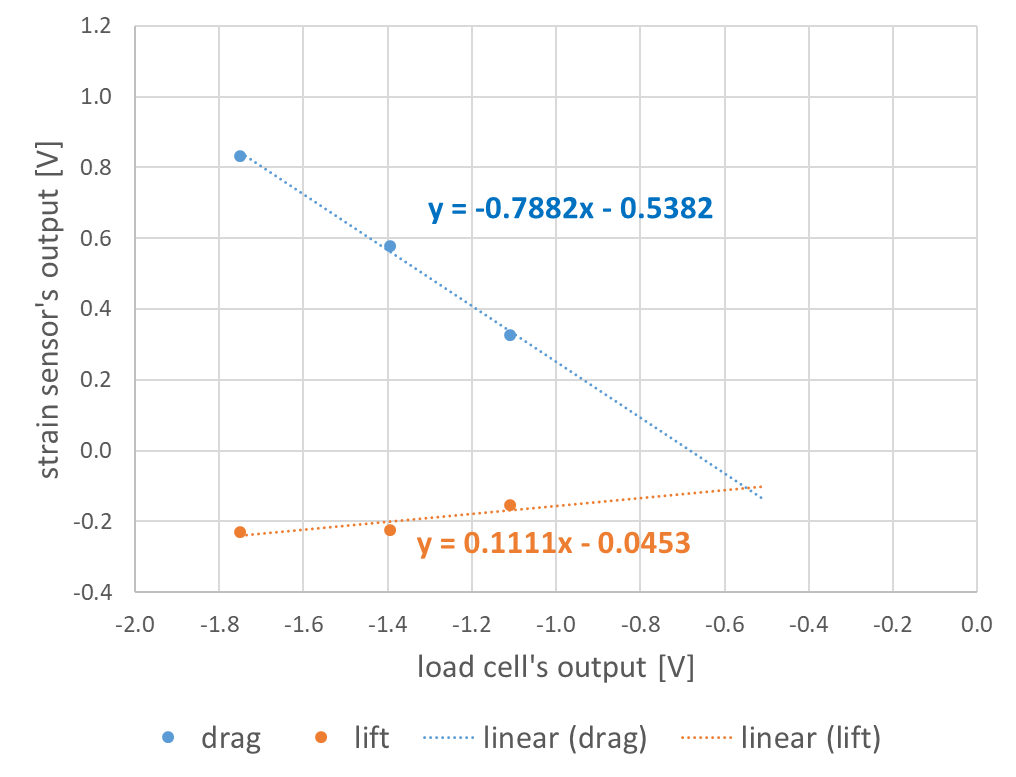
\includegraphics[width=68mm]{../images/graph_21119_drag_previous.png}
        \caption{Previous data of load cell - strain sensors (drag)}
        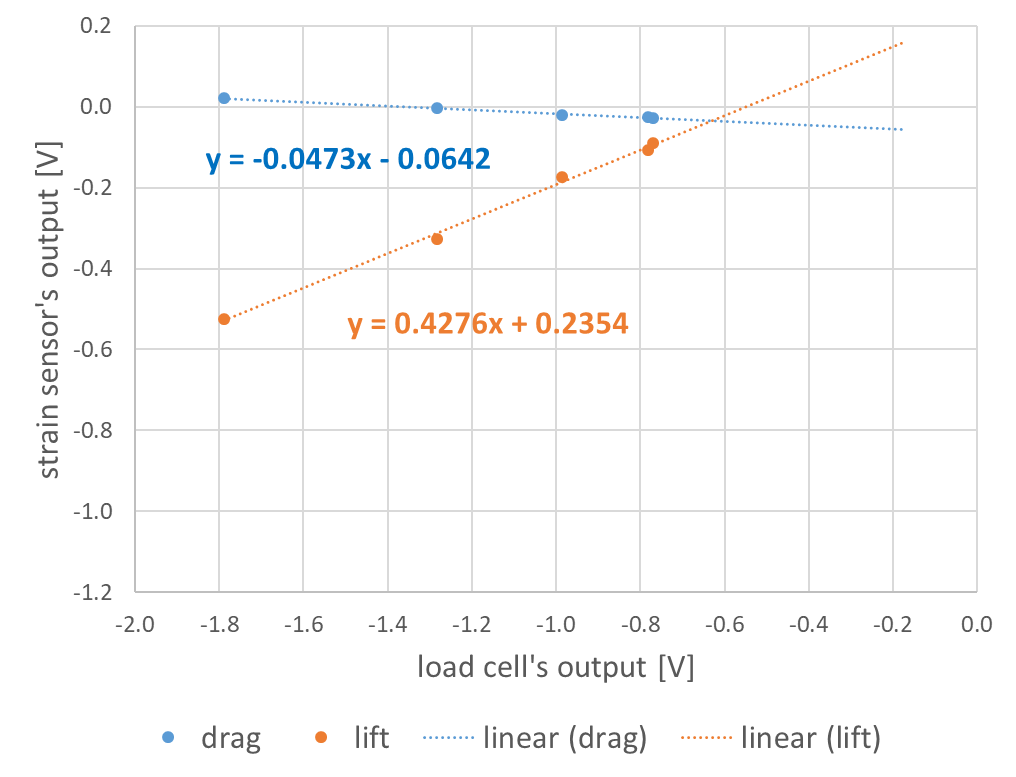
\includegraphics[width=68mm]{../images/graph_21119_lift_previous.png}
        \caption{Previous data of load cell - strain sensors (lift)}
    \end{center}
\end{figure}

\newpage

\subsection{再実施結果:抗力}
以下のFig.4~Fig.6に抗力方向の実験データを示す.
なお,ロードセルを測定ごとに再設置し実験を行った.
また,データは,採用点と後部の9点の計10点(10秒間)の平均を用いている.
\begin{figure}[htbp]
    \footnotesize
    \begin{center}
        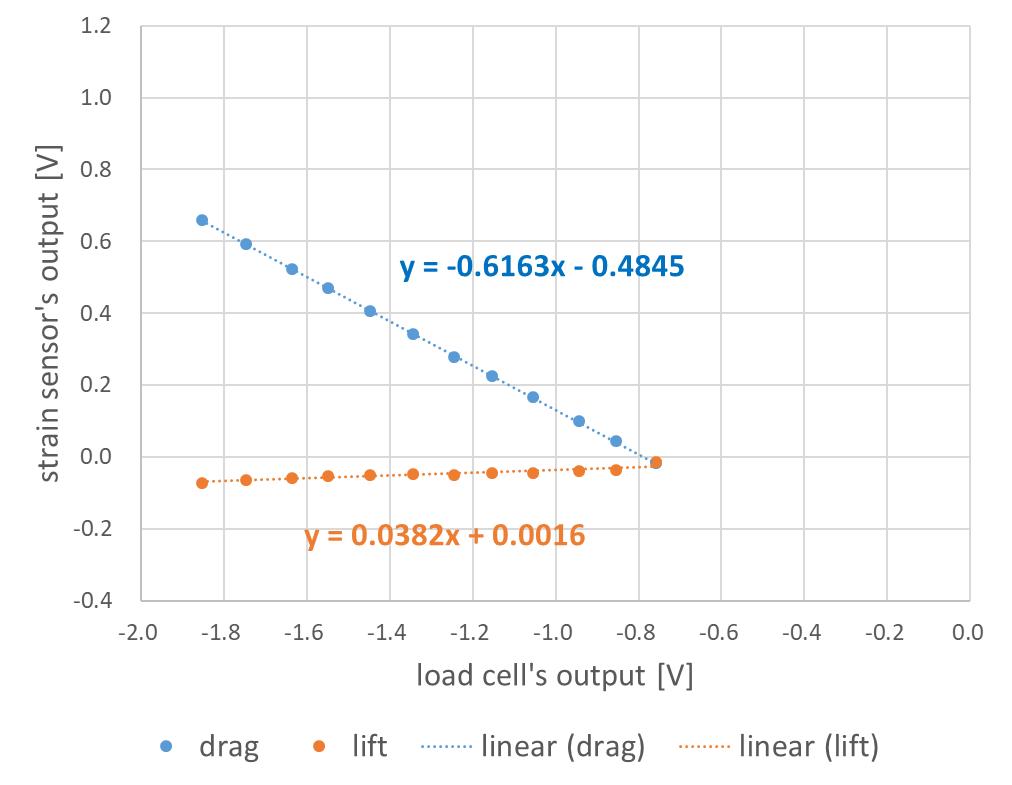
\includegraphics[width=68mm]{../images/graph_21119_drag_1.png}
        \caption{Re-experimental data of drag (1)}
        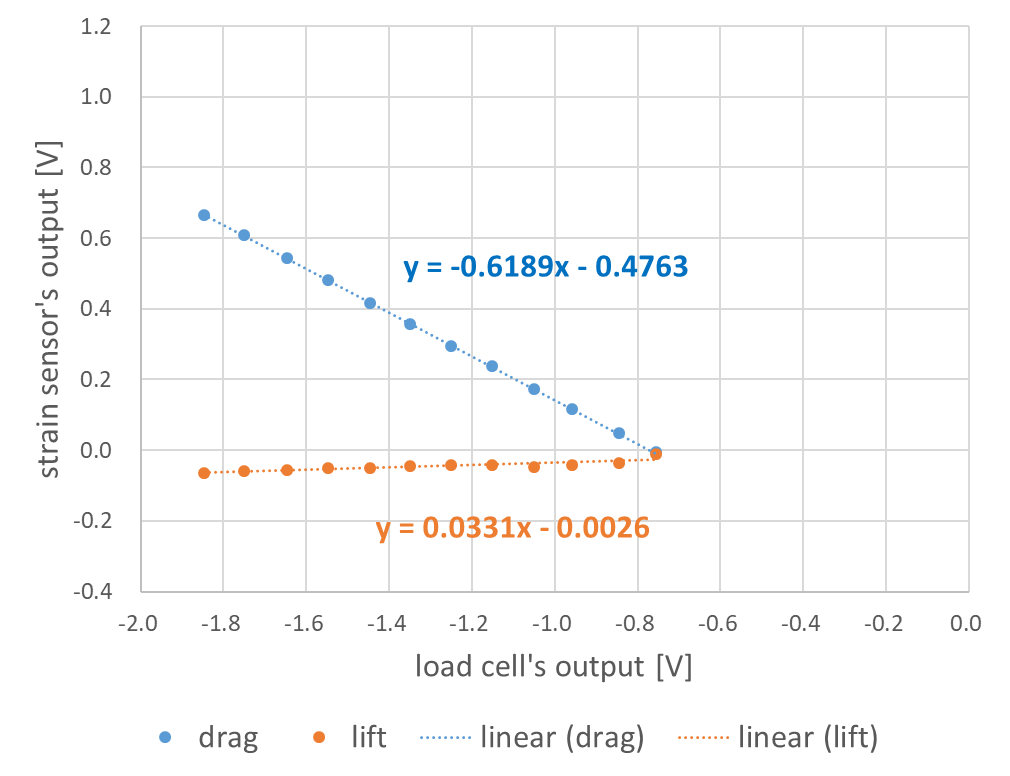
\includegraphics[width=68mm]{../images/graph_21119_drag_2.png}
        \caption{Re-experimental data of drag (2)}
        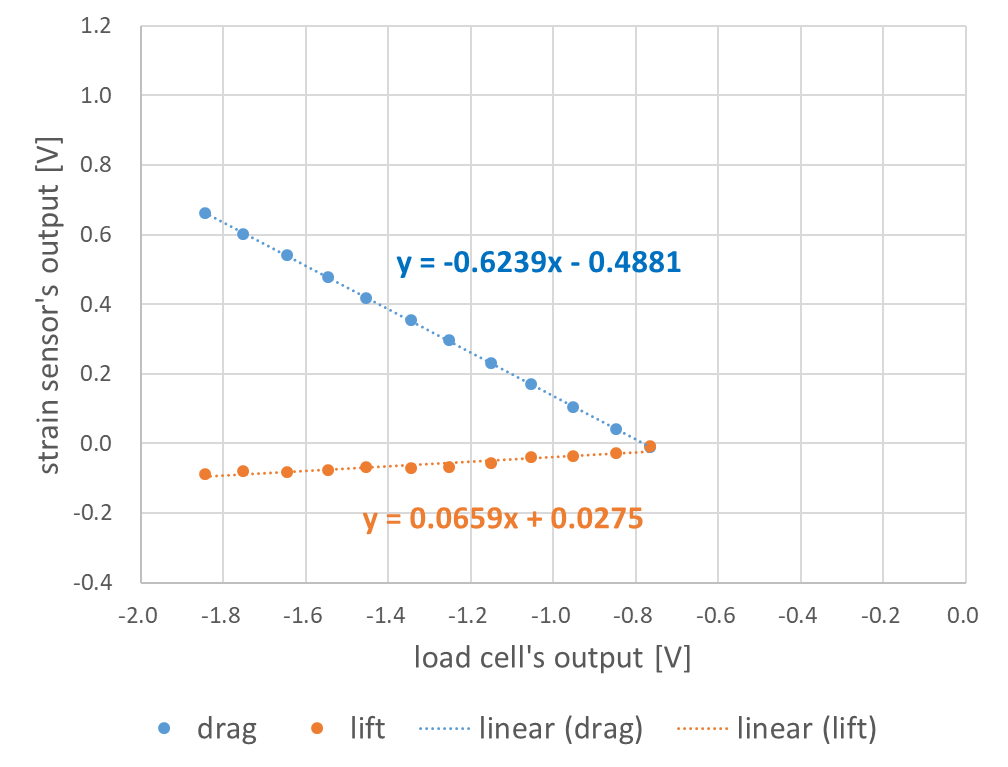
\includegraphics[width=68mm]{../images/graph_211111_drag_3.png}
        \caption{Re-experimental data of drag (3)}
    \end{center}
\end{figure}

\newpage

\subsection{再実施結果:揚力}
以下のFig.7~Fig.9に揚力方向の実験データを示す.
実験条件及びデータ解析方法は抗力方向と同様である.
\begin{figure}[htbp]
    \footnotesize
    \begin{center}
        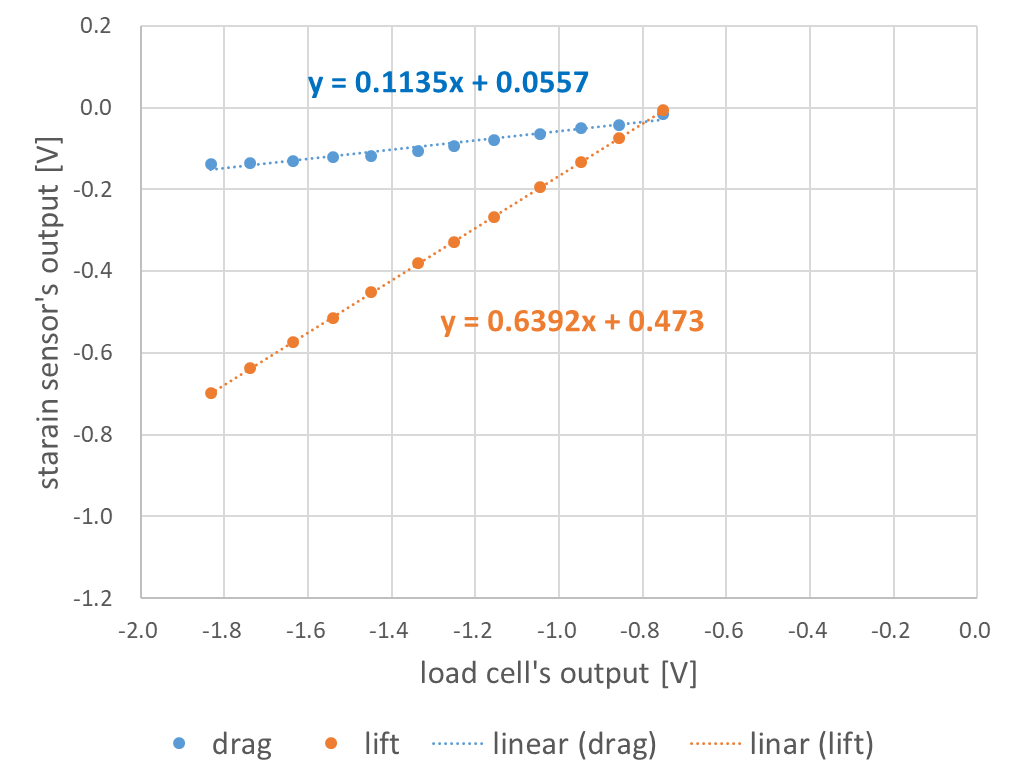
\includegraphics[width=68mm]{../images/graph_21119_lift_1.png}
        \caption{Re-experimental data of lift (1)}
        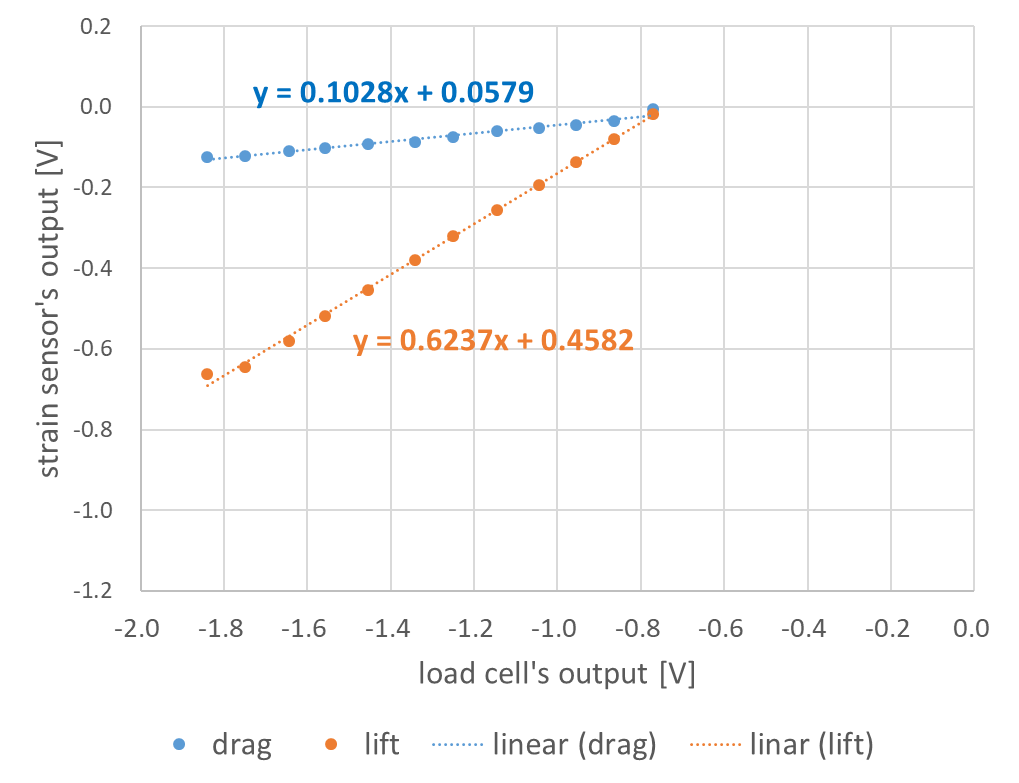
\includegraphics[width=68mm]{../images/graph_21119_lift_2.png}
        \caption{Re-experimental data of lift (2)}
        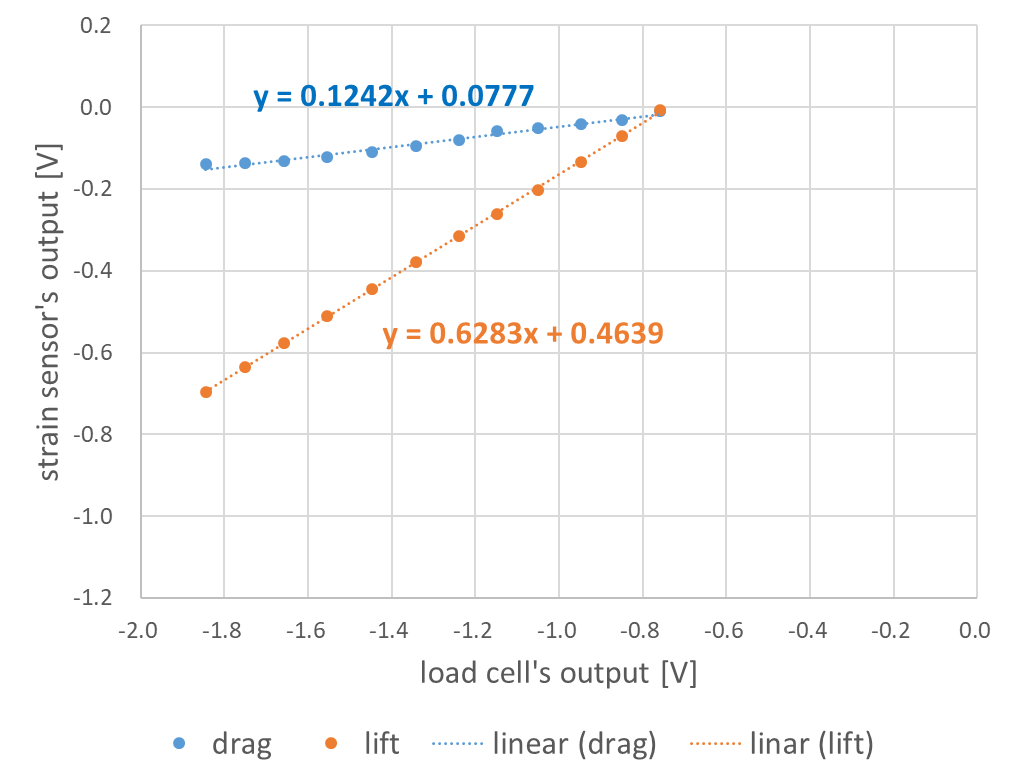
\includegraphics[width=68mm]{../images/graph_21119_lift_3.png}
        \caption{Re-experimental data of lift (3)}
    \end{center}
\end{figure}

\newpage

\subsection{結果分析}
再実験結果(Fig.4~Fig.9)をそれぞれ比較すると,
3回の実験データには同様の傾向が確認できる.\par
しかし,以前の実験結果(Fig.2,Fig.3)と比較すると
近似直線の傾きに大きな差異があり,
目的とは異なる方向(例:抗力方向に作用力を加えた場合の揚力方向の出力電圧)
の出力についても異なる傾向があることがわかる.

\section{オフセット値の考慮}
実験結果から,”原点を通らない”近似直線が算出されたことから,
ロードセルのストレインアンプの出力電圧にオフセットがあると仮定した.
そのオフセット値を,実験結果のロードセルの出力電圧から差し引いた値を
採用することとする.\\

\begin{figure}[htbp]
    \footnotesize
    \begin{center}
        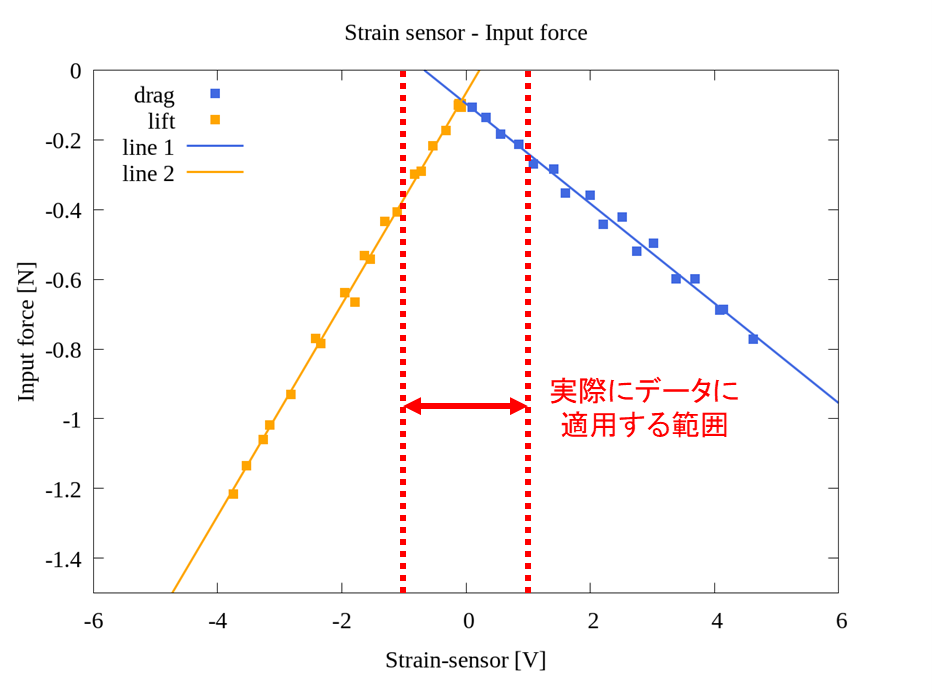
\includegraphics[width=80mm]{../../2110/images/image_08.png}
        \caption{Range to use}
        \vskip\baselineskip
        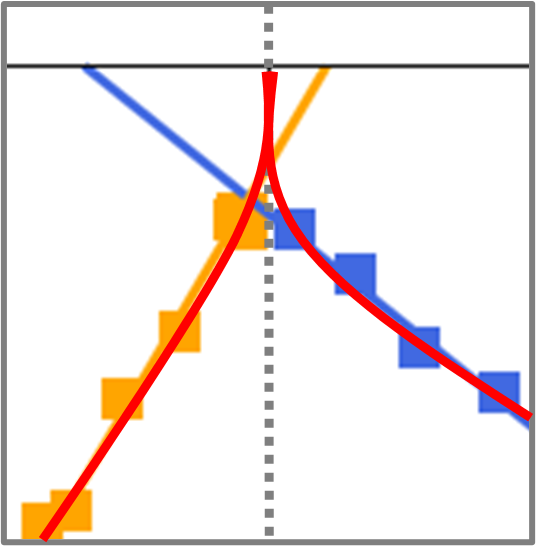
\includegraphics[width=30mm]{../../2110/images/image_10.png}
        \caption{Non-linear region}
    \end{center}
\end{figure}

\newpage

\subsection{オフセット値の算出}
実験の際にロードセルのストレインアンプは,
バランスをとった後,0.720付近の値を示すことが多くある.
そこで,ロードセルに作用力が加えられていない状態の出力電圧を測定し,
その平均値をオフセット値として採用することとした.
算出したオフセット値は以下のようになった.
今回は,60秒間の測定値の平均を採用した.
\begin{eqnarray*}
  \mathrm{offset} = -0.728
\end{eqnarray*}

\subsection{オフセット値の適用}
算出したオフセット値を以前の実験結果に適用した.\\

\subsubsection*{オフセット値適用前の実験結果}
以下のFig.12,Fig.13にストレインアンプのオフセット値適用前の実験結果を示す.
\begin{figure}[htbp]
    \footnotesize
    \begin{center}
        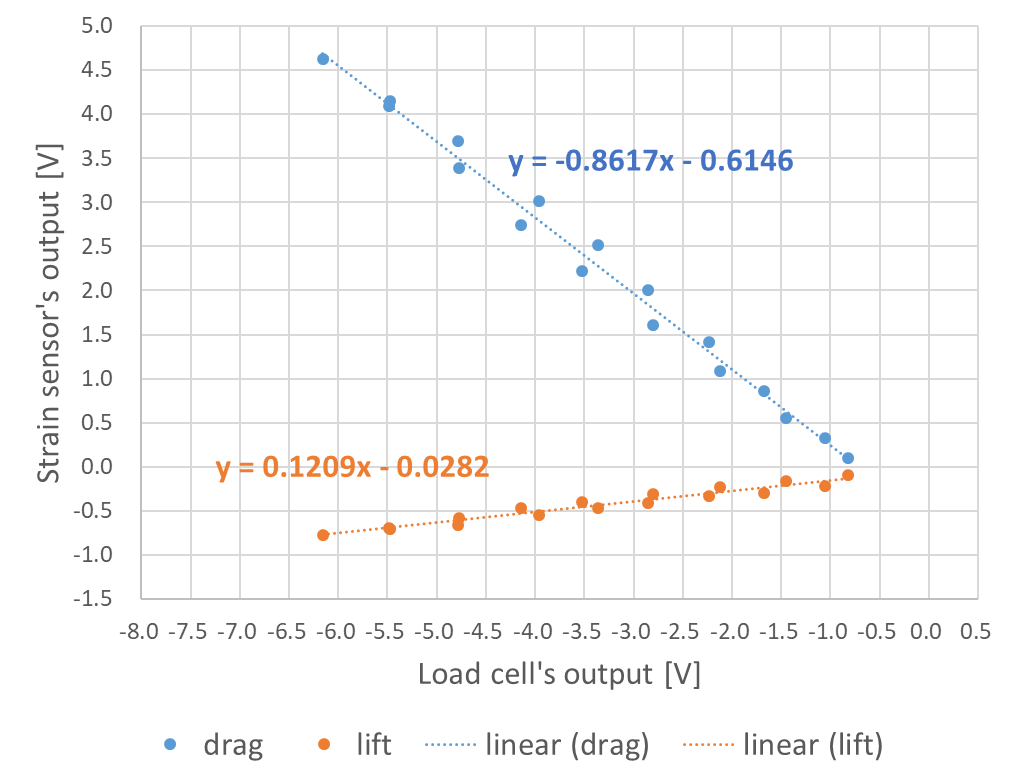
\includegraphics[width=72mm]{../images/calibration_2_drag.png}
        \caption{Result of load cell - strain sensor (drag)}
        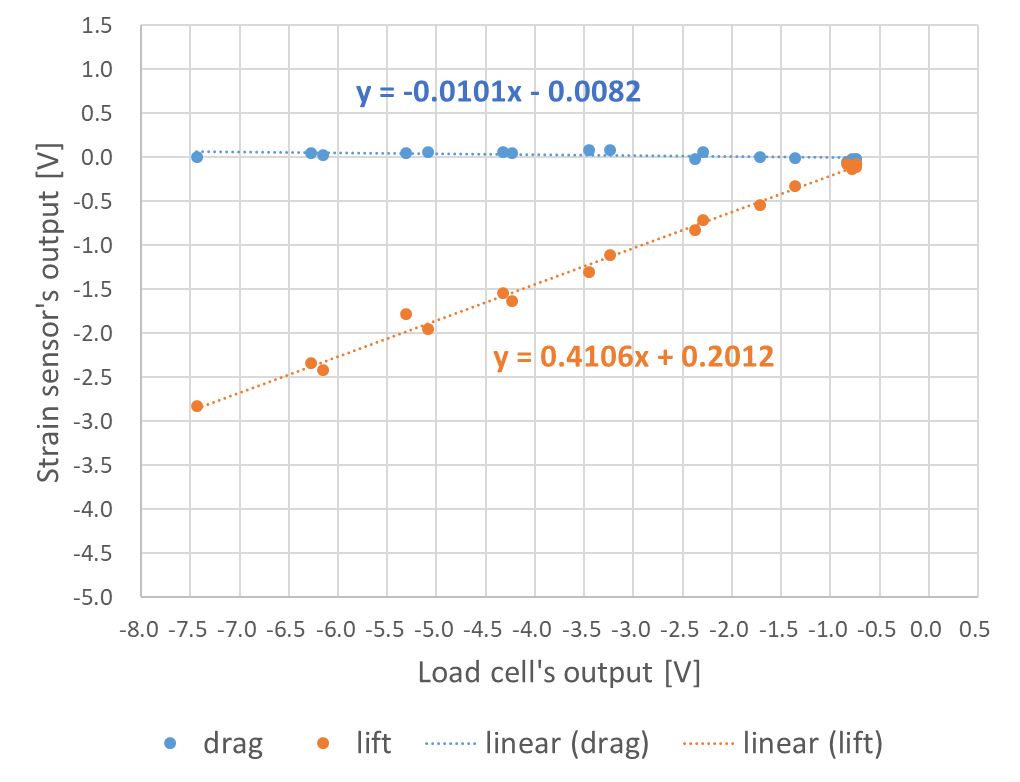
\includegraphics[width=72mm]{../images/calibration_2_lift.png}
        \caption{Result of load cell - strain sensor (lift)}
    \end{center}
\end{figure}

\newpage

\subsubsection*{オフセット値適用後の実験結果}
以下のFig.14,Fig.15にストレインアンプのオフセット値適用後の実験結果を示す.\par
\begin{figure}[htbp]
    \footnotesize
    \begin{center}
        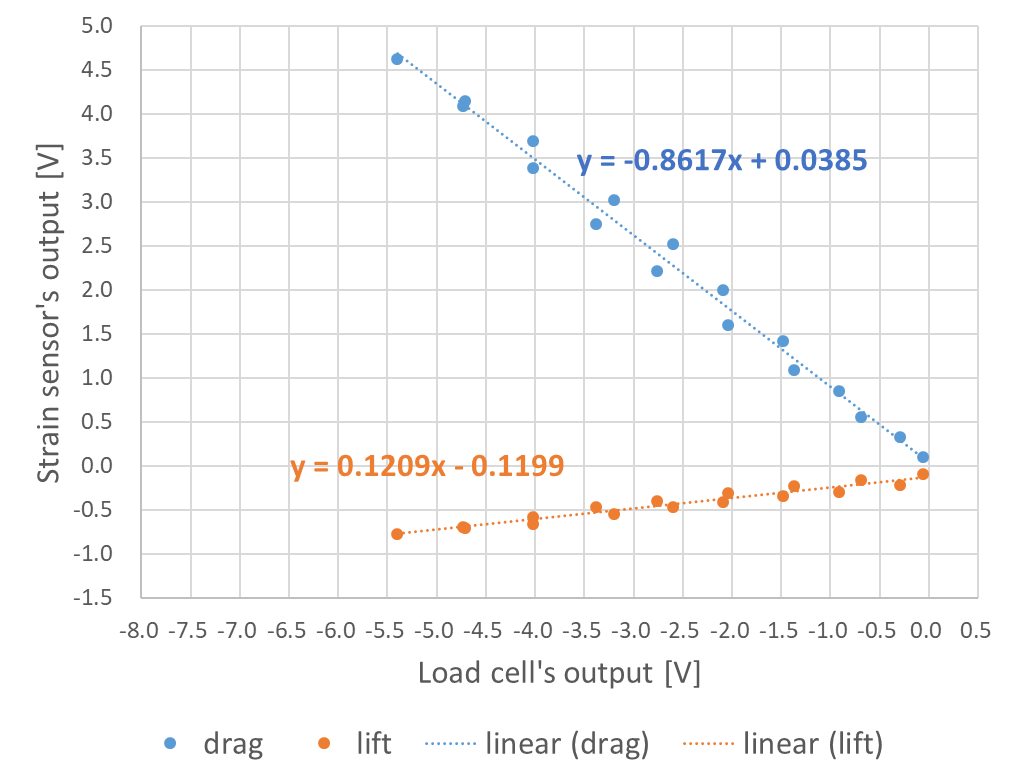
\includegraphics[width=72mm]{../images/calibration_2_drag_offset.png}
        \caption{Considered offset value (drag)}
        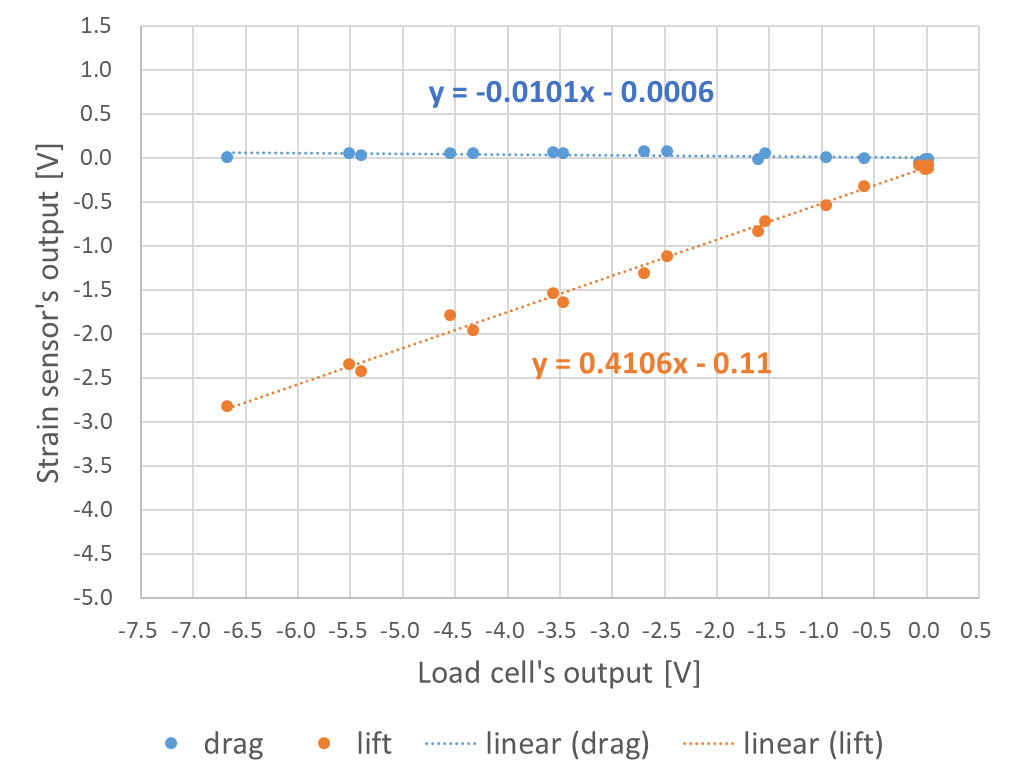
\includegraphics[width=72mm]{../images/calibration_2_lift_offset.png}
        \caption{Considered offset value (lift)}
    \end{center}
\end{figure}

\subsubsection*{結果分析}

抗力方向の校正実験結果であるFig.12とFig.14及び,
揚力方向の校正実験結果であるFig.13とFig.15を比較すると,
算出したオフセット値を適用することで近似直線の開始点が原点に近づいていることがわかる.

\newpage

\subsection{校正実験結果を用いた換算式の算出}
同様に,入力荷重とひずみセンサの出力電圧の関係についての結果を以下のFig.16,Fig.17に示す.
なお,Fig.16はFig.1,Fig14の結果,Fig.17はFig.1,Fig15の結果を利用している.
\begin{figure}[htbp]
    \footnotesize
    \begin{center}
        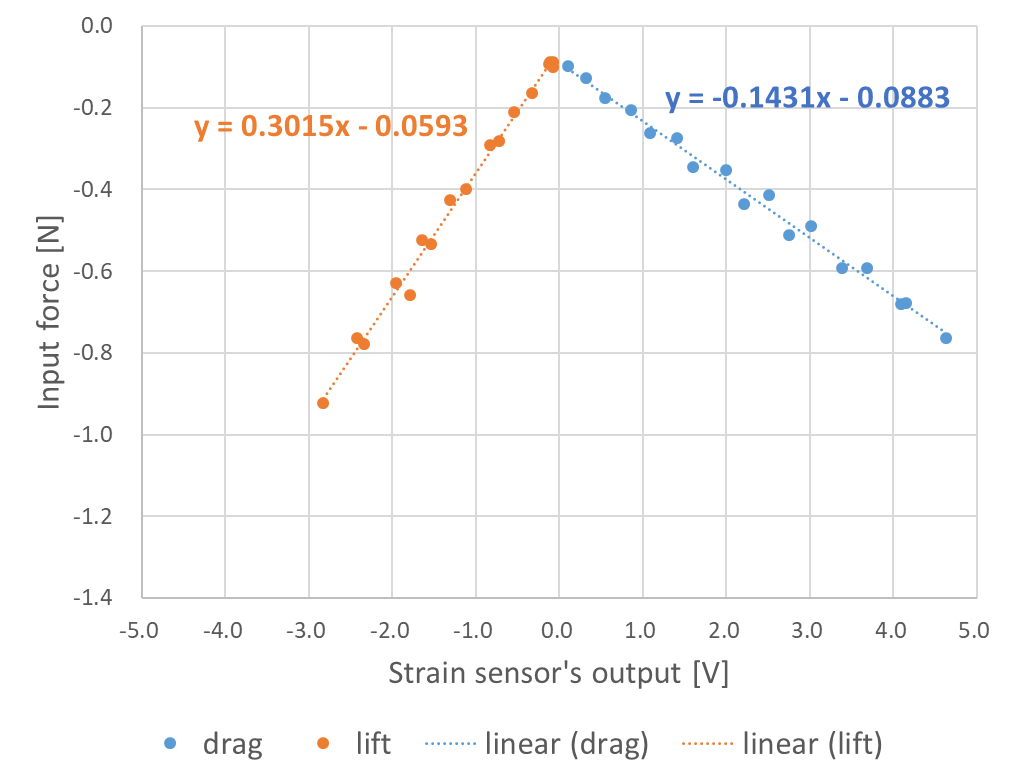
\includegraphics[width=72mm]{../images/convert.png}
        \caption{Correlation between input force and output voltage}
        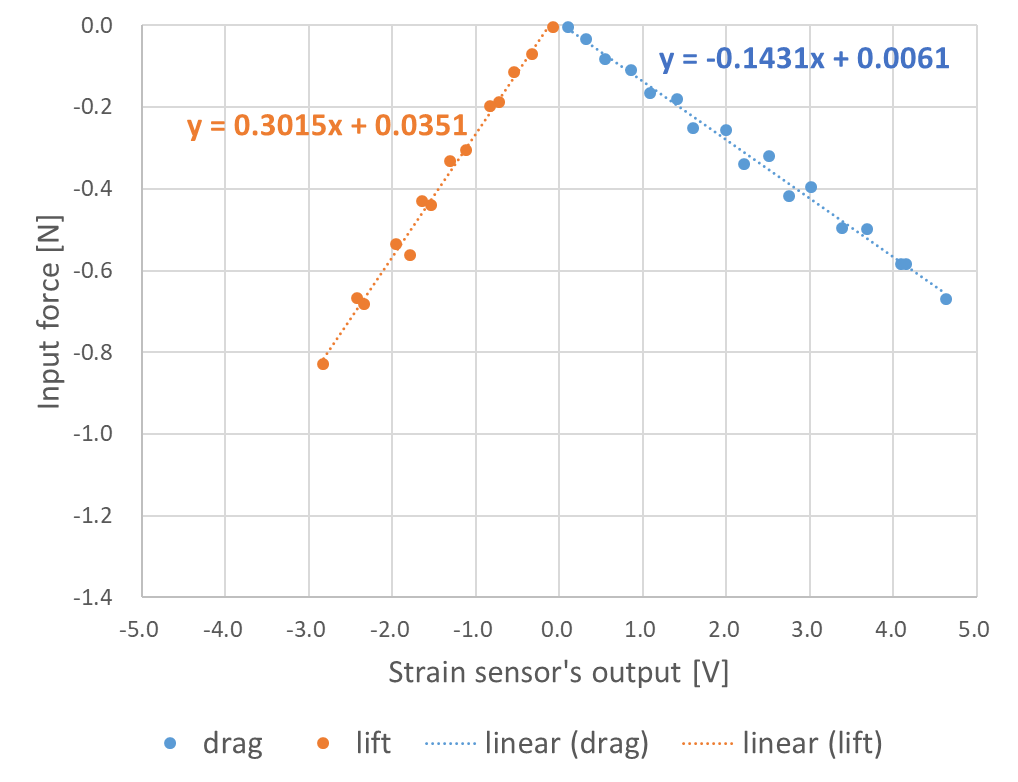
\includegraphics[width=72mm]{../images/convert_offset.png}
        \caption{Considered offset values}
    \end{center}
\end{figure}

\vskip\baselineskip

\subsubsection*{結果分析}

オフセット値の適用前(Fig.16)とオフセット値適用後(Fig.17)を比較すると,
こちらもオフセット値を適用することで近似直線の開始点が原点に近づいていることが確認できる.\par
したがって,ロードセルに用いているストレインアンプについては,
バランスをとった後でも,実験結果にオフセット値を適用しなければならないことがわかった.

\newpage

\section{卒業研究について}

現在のタイヤモデルの作用力測定について,
荷重と出力電圧の関係を校正実験から得る必要がある.
ここで,抗力・揚力の2方向からの作用力の関係を
正しく評価することが非常に困難であり,
ひずみセンサの取付方法や取付部の断面形状によって
揚力と抗力に依存性が生じている可能性があると考えた。\par
したがって、今後の研究テーマとして、
ひずみセンサを用いた2方向の作用力の評価方法について取り上げることとした。\\

\subsection{研究目的}
    $x$軸,$y$軸方向に取り付けられたひずみセンサについて,
    作用力の方向による出力電圧への影響・取付部の断面形状の違いによる影響を調べ,
    その関係から作用力実験結果の出力電圧を荷重に適切に変換する方法を模索し提案することを目的とする.
    \par
    また,その結果から選定された断面形状の取付部を高感度ひずみセンサを用いて作成し,
    現在使用しているひずみセンサとの比較実験を行うことで,その改善結果を示す.\\

\subsection{研究方針}
    \begin{enumerate}[(1)]
        \item 従来の実験装置について,作用力の方向による出力電圧の変化を調べる.
        \item [$\rightarrow$] 現在の実験装置の特徴を理解し,
              これまでの出力電圧から作用力への変換課程における問題点を明確にする.
        \item (1)の実験について,異なる幾つかの断面形状で実験を行い,
              出力電圧のひずみセンサ取付部の断面形状による違いを調べる.
        \item [$\rightarrow$] 断面形状の違いがどのような影響を及ぼすのかを明らかにし,
              2ゲージ法での測定の際に望ましい断面形状を提案する.
        \item (2)の結果より選定された断面形状の取付部を高感度ひずみセンサを用いて作成し,
              再度同様の実験を行う.
        \item [$\rightarrow$] 現在使用しているひずみセンサとの比較実験を行うことで,
              その改善結果を示す.
    \end{enumerate}

\newpage
\subsection{比較実験の対象}
ひずみゲージ取付部の断面形状の違いによる影響を調べるため,
以下の3種の断面形状について,比較実験を行う.\par
\begin{enumerate}[(i)]
    \item 円筒  (外形:$D_1=$20.0[mm],内径:$D_2=$18.0[mm])
    \item 円   (直径:$D$)
    \item 正方形(辺の長さ:$L$)
\end{enumerate}
\begin{figure}[htbp]
    \footnotesize
    \begin{center}
        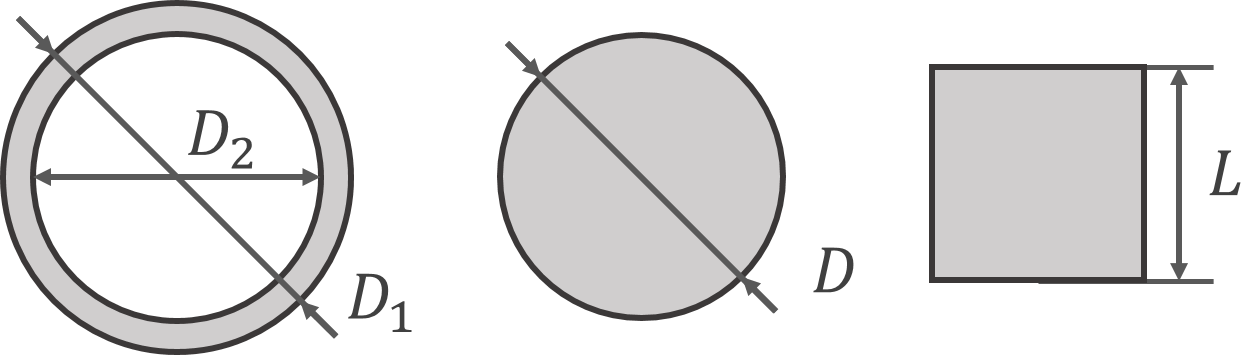
\includegraphics[width=80mm]{../images/testpieces_2.png}
        \caption{Cross-sectional shape of test pieces}
    \end{center}
\end{figure}
なお,現在の実験装置で使用されている (1)円筒を基準とし,
同等の断面二次モーメントを持つ形状とした.\\

\subsection{断面二次モーメントの算出}
(i)の円筒を基準に算出した断面二次モーメントを以下に示す.
なお,上記の”比較実験の対象”の記号に対応している.

\subsubsection{算出結果}
\begin{screen}
    \begin{enumerate}[(i)]
        \item 円柱 $\cdots$ $D_1=\;$20.0 [mm],$D_2=\;$18.0 [mm]
        \item 円筒 $\cdots$ $D=\;$15.3 [mm]
        \item 角柱 $\cdots$ $L=\;$13.4 [mm]
    \end{enumerate}
\end{screen}

\subsubsection{算出過程}
    \begin{itembox}[l]{円の断面二次モーメント}
        \begin{center}
            $\displaystyle I = \frac{\pi}{64}D^4\;\left(D:直径\right)$
        \end{center}
    \end{itembox}
    \begin{itembox}[l]{正方形の断面二次モーメント}
        \begin{center}
            $\displaystyle I = \frac{1}{12}L^4\;\left(L:辺の長さ\right)$
        \end{center}
    \end{itembox}

    \newpage
    
    \begin{enumerate}[(i)]
        \item 円筒(外形:$D_1=$20.0[mm],内径:$D_2=$18.0[mm])\\
        $\blacksquare$ 断面二次モーメントの算出
        \begin{eqnarray*}
            I &=& \frac{\pi}{64} \left(20^4 - 18^4\right)\\
            &=& \frac{\pi}{64} × 55024\\
            &=& 2700.98 \dots\\
            &\approx& 2701.0 \left[\mathrm{mm^4}\right]
        \end{eqnarray*}
        \item 円(直径:$D$)\\
        $\blacksquare$ 直径の算出 
        \begin{eqnarray*}
            I &=& \frac{\pi}{64}D^4\\
            \frac{\pi}{64} × 55024 &=& \frac{\pi}{64}D^4\\
            D^4 &=& 55024\\
            D&=& 15.31\dots\\
            &\approx& 15.3 \left[\mathrm{mm}\right]
        \end{eqnarray*}
        \item 正方形(辺の長さ:$L$)\\
        $\blacksquare$ 辺の長さの算出
        \begin{eqnarray*}
            I &=& \frac{1}{12}L^4\\
            2701.0 &=& \frac{1}{12}L^4\\
            L^4 &=& 2701.0 * 12\\
            &=& 32412\\
            L&=& 13.41\dots\\
            &\approx& 13.4 \left[\mathrm{mm}\right]
        \end{eqnarray*}
    \end{enumerate}

    \subsection{実験装置のたわみ量とひずみの算出}
    試験用のひずみセンサを選定するにあたり,
    ひずみセンサの取付部の作用力によるひずみ量を調べる必要がある.
    ここで,簡単のため可能な限り切りのいい数字を使っておおよその変位量を算出した.
    \begin{figure}[htbp]
        \footnotesize
        \begin{center}
            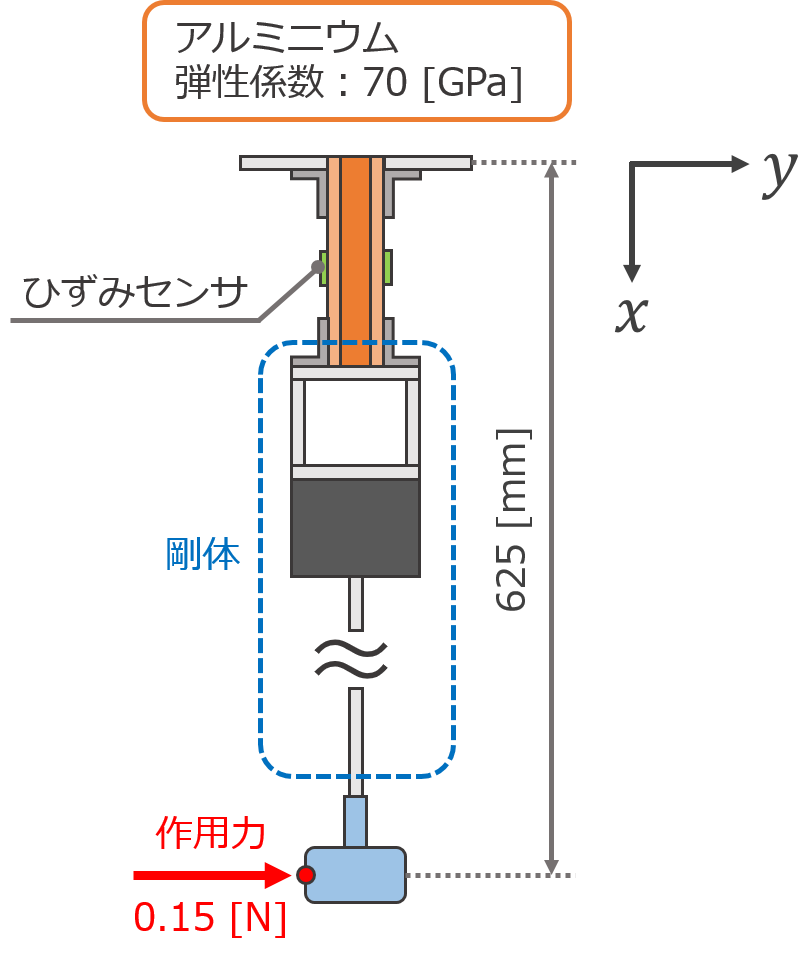
\includegraphics[width=60mm]{../images/moment.png}
            \caption{Cross-sectional shape of experimental device}
        \end{center}
    \end{figure}\\

\newpage

    \subsubsection{算出結果}
        \begin{screen}
            \begin{itemize}
                \item 先端のたわみ量  :$0.151 \;\left[\mathrm{mm}\right]$
                \item 取付軸表面の伸縮量:$1.029 × 10^{-3} \;\left[\mathrm{mm}\right]$
                \item 取付軸表面のひずみ:$5.717 × 10^{-6} \left[\mathrm{-}\right]$
            \end{itemize}
        \end{screen}
    
    \vskip\baselineskip

    \subsubsection{算出条件}
    \begin{screen}
        \begin{itemize}
            \item [$\bullet$] アルミニウムの弾性係数  :$E = 70 \left[\mathrm{GPa}\right]$
            \item [$\bullet$] ひずみセンサと作用点の距離:$l_1 = 725 \left[\mathrm{mm}\right]$
            \item [$\bullet$] 取付部材料の長さ     :$l_2 = 180 \left[\mathrm{mm}\right]$
            \item [$\bullet$] 作用力          :$F = 0.15 \left[\mathrm{N}\right]$              
            \item [$\bullet$] 断面二次モーメント    :$I = 2701 \left[\mathrm{mm^4}\right]$              
            \item [$\bullet$] 取付部に加わるモーメント :$M$              
            \item [$\bullet$] 取付部のたわみの曲率半径 :$R$              
            \item [$\bullet$] 取付部のたわみ角     :$\theta$
            \item [$\bullet$] 取付部のたわみ      :$w$
            \item [$\bullet$] 取付部表面の伸び     :$\lambda$
            \item [$\bullet$] 取付部表面のひずみ    :$\varepsilon$
            \item [$\bullet$] 取付部表面と中立軸の距離 :$\delta r$              
        \end{itemize}
    \end{screen}
    
    \subsubsection{算出過程}
    \begin{itemize}
        \item [$\blacksquare$] 実験装置に加わるモーメントの算出
        \begin{eqnarray*}
            M &=& F × \frac{l_1}{1000}\\
            &=& 0.15 × 0.725\\
            &=& 0.10875 \;\left[\mathrm{N \cdot m}\right]
        \end{eqnarray*}
        \item [$\blacksquare$] たわみの曲率半径の算出
        \begin{itembox}[l]{たわみの曲率半径}
            \begin{center}
                $\displaystyle \frac{1}{R} = \frac{M}{EI}$
            \end{center}
        \end{itembox}
        \begin{eqnarray*}
            R &=& \frac{EI}{M}\\
            &=& 70 × 2701 × \frac{100000}{10875}\\
            &\approx& 1738574.713 \left[\mathrm{mm}\right]
        \end{eqnarray*}
        \item [$\blacksquare$] 位置$x$[mm] におけるたわみ角とたわみの算出
        \begin{itembox}[l]{たわみの微分方程式}
                \begin{center}
                    $\displaystyle \frac{d^2w}{dx^2}=-\frac{M}{EI}$\\
                    \vskip\baselineskip
                    ※ 今回のひずみは正の値となる
                \end{center}
        \end{itembox}
        \begin{itembox}[l]{初期条件}
        \begin{itemize}
            \item [$\bullet$] $x=0$ のとき $w=0$,$\theta =0$
        \end{itemize}
        \end{itembox}
        \begin{eqnarray*}
            \frac{d^2w}{dx^2}&=&\frac{M}{EI}\\
            &=&\frac{0.10875}{70 × 2701}\\
            &=&5.7518 \cdots × 10^{-7}\\
            &\approx& 5.752 × 10^{-7} \;\left[\mathrm{1/mm}\right]\\ \\
            \frac{dw}{dx} &=& \theta = \frac{M}{EI} x + C_1\\ \\
            w &=& \frac{1}{2} \frac{M}{EI} x^2 + C_1x + C_2
        \end{eqnarray*}
        初期条件より
        \begin{eqnarray*}
            C_1 = C_2 = 0
        \end{eqnarray*}
        したがって,
        \begin{eqnarray*}
            \theta &=& \frac{M}{EI}x\\ \\
            w &=& \frac{1}{2}\frac{M}{EI}x^2\\
        \end{eqnarray*}
            \item [$\blacksquare$] ひずみセンサ取付部($x=90$)の伸びの算出\\
        $x = 90$のとき,たわみ角は,
        \begin{eqnarray*}
            \theta &=& \frac{M}{EI} × 90\\
            &=& 5.7152 × 10^{-7} × 90\\
            &=& 5.1437 × 10^{-5}\\
            &\approx& 5.144 × 10^{-5} \;\left[\mathrm{rad}\right]
        \end{eqnarray*}
        したがって,取付軸の伸び$\lambda$は,
        \begin{eqnarray*}
            \lambda &=& \left(R+\delta r\right)\theta - R\theta\\
            &=& \delta r \theta\\
            &=& 20 × \;\theta\\
            &=& 20 × 5.1437 × 10^{-5}\\
            &=& 1.02874 × 10^{-3}\\
            &\approx& 1.029 × 10^{-3} \;\left[\mathrm{mm}\right]\\
        \end{eqnarray*}
        \item [$\blacksquare$] ひずみセンサ取付部($x=90$)のひずみの算出
            \begin{eqnarray*}
                \varepsilon &=& \frac{\lambda}{l_2}\\
                &=& \frac{1.029 × 10^{-3}}{180}\\
                &=& 5.7166 \cdots × 10^{-6}\\
                &\approx& 5.717 × 10^{-6} \left[\mathrm{-}\right]
            \end{eqnarray*} 
        \item [$\blacksquare$] 先端($x=725$)のたわみ量 $w$ の算出
        \begin{eqnarray*}
            w &=& \frac{1}{2} × \frac{M}{EI} × l^2\\
            &=& \frac{1}{2} × 5.752 × 10^{-7} × 725^2\\
            &=& 0.1511 \cdots\\
            &\approx& 0.151 \;\left[\mathrm{mm}\right]
        \end{eqnarray*} 
    \end{itemize}

\section{実験装置の製作}
作用力方向の違いによる影響を調べるため、
現在の実験装置を用いて仮実験を行うこととした。
仮実験を行うにあたり,以下のFig.20 の実験装置を作成した。
\begin{figure}[htbp]
    \footnotesize
    \begin{center}
        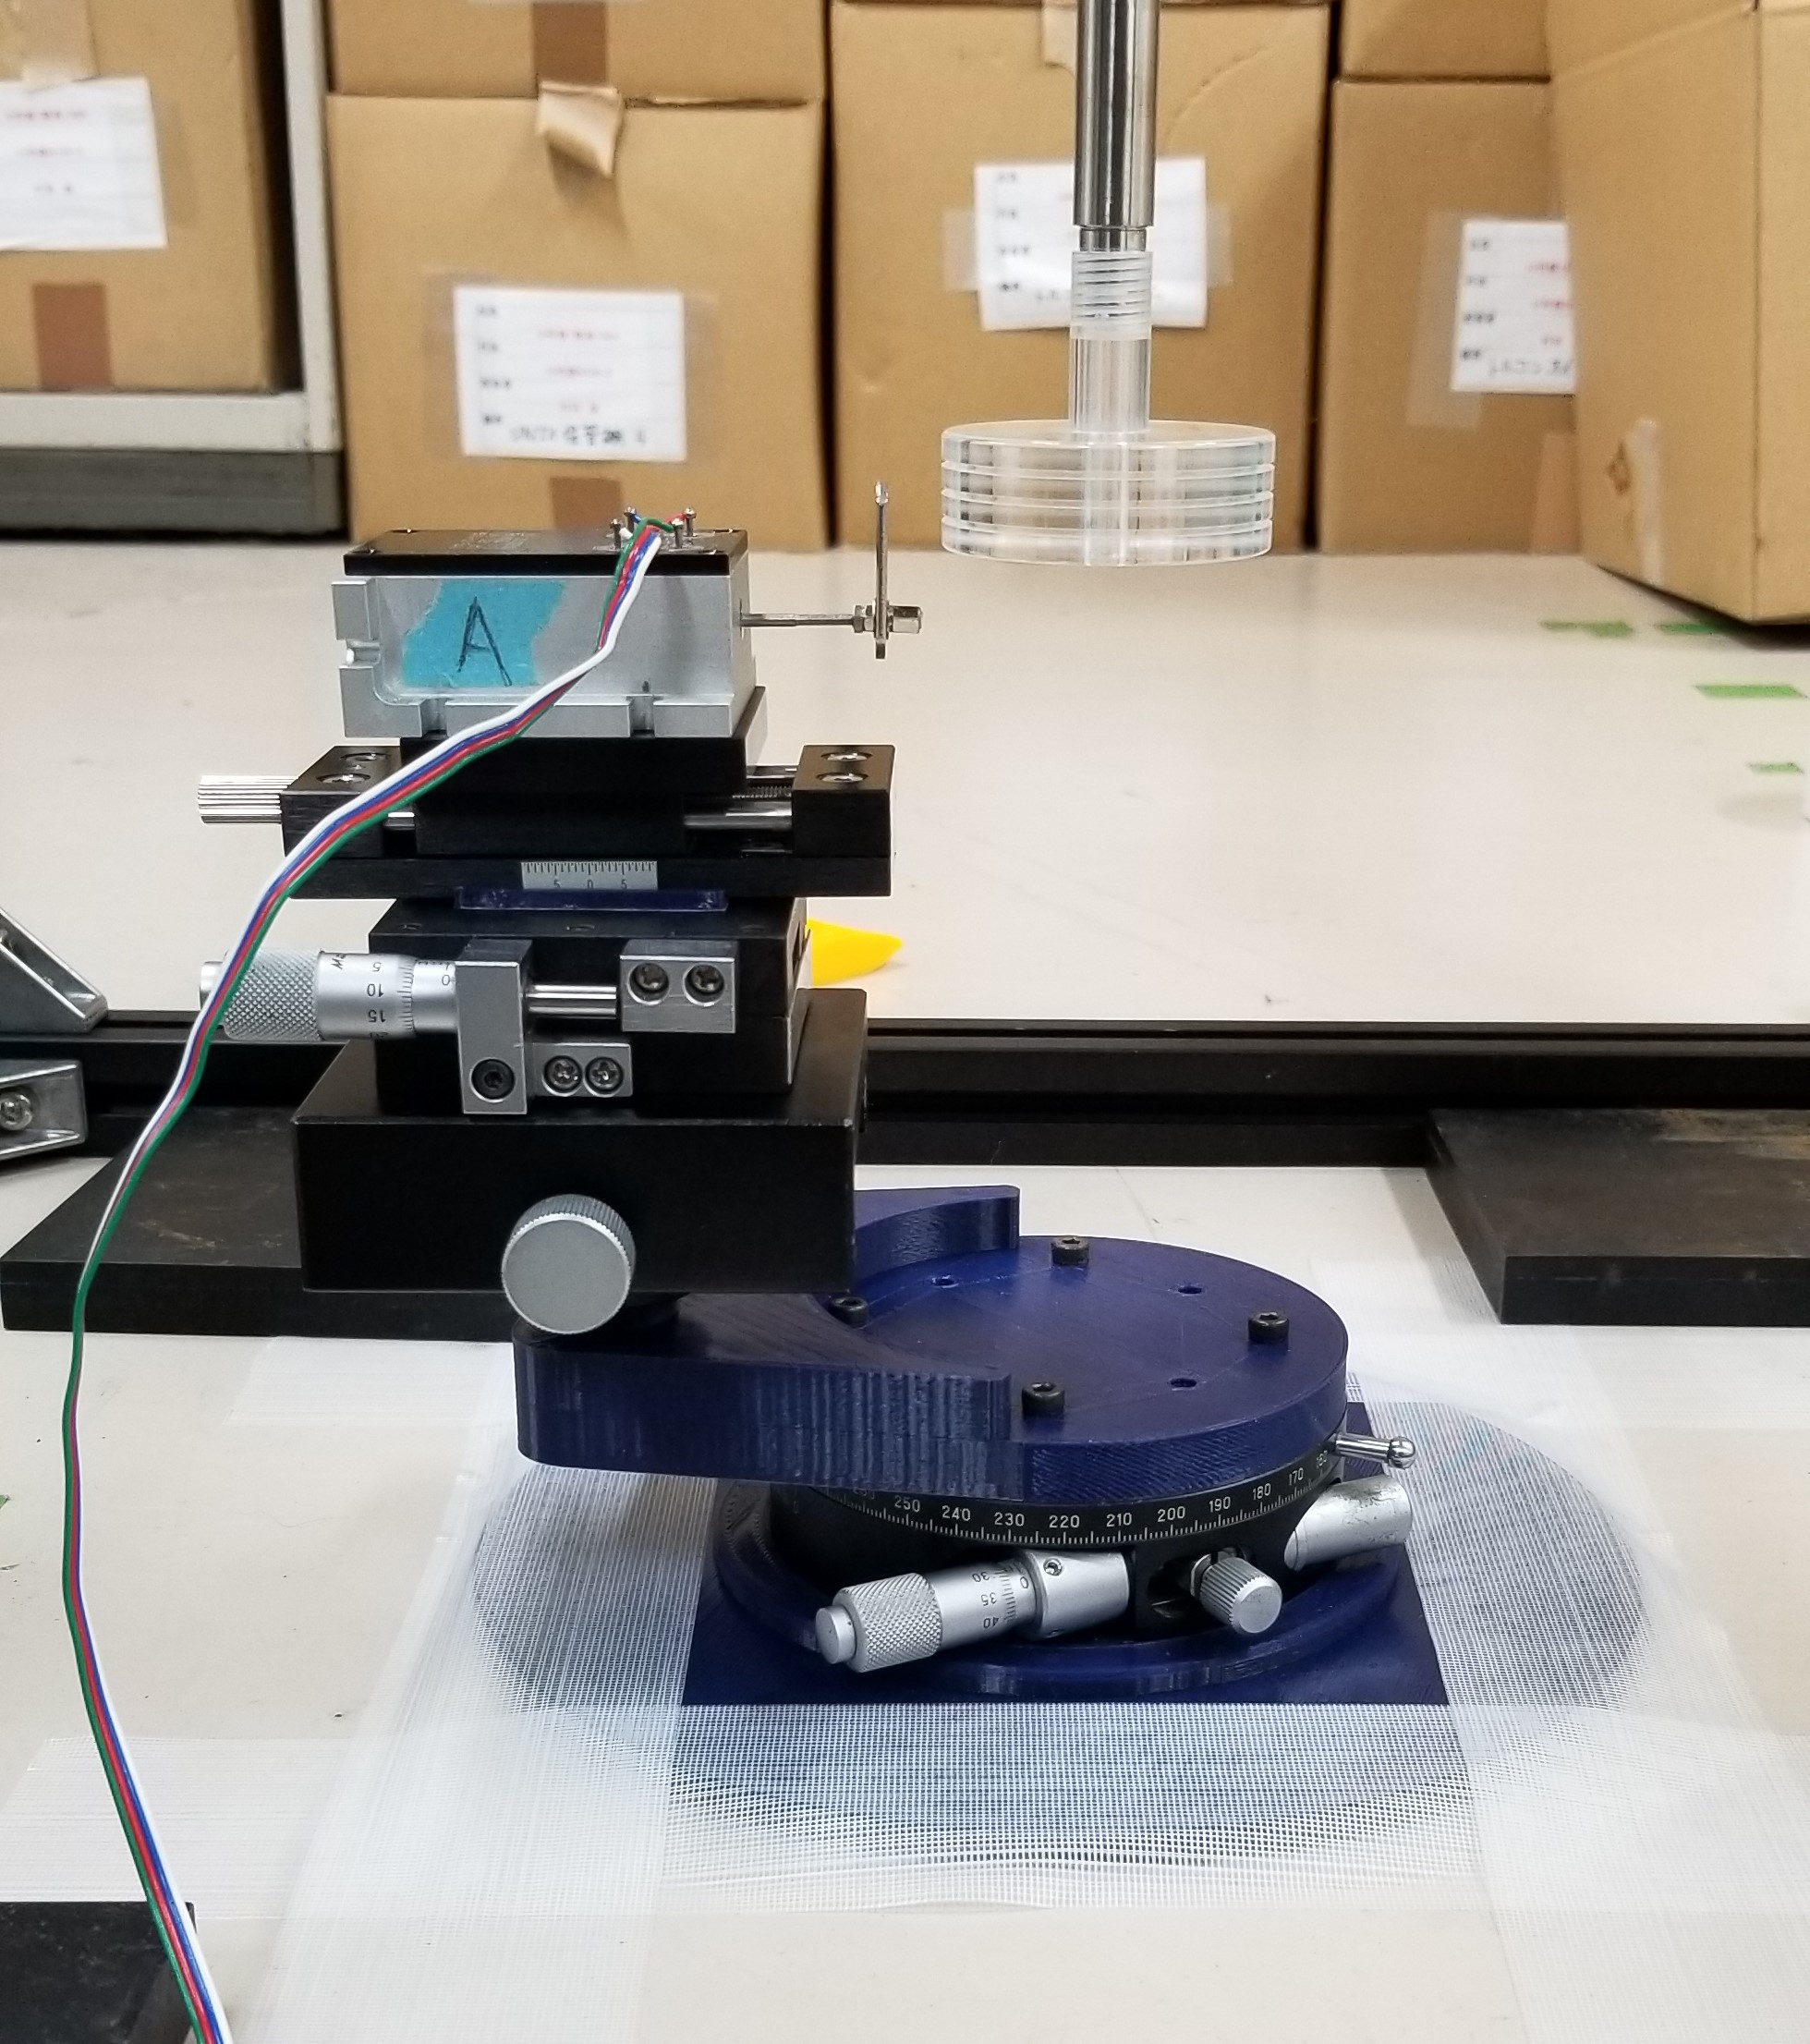
\includegraphics[width=80mm]{../images/device_1.jpg}
        \caption{Experimental device}
    \end{center}
\end{figure}

\newpage

\section{実験結果}
作成した実験装置を用いて、試験的に実験を行った。
その結果を以下に示す。

\newpage

\section{今月の進捗と12月の予定}
\begin{itemize}
    \item [$\blacksquare$] 今月の進捗
    \begin{itemize}
        \item [$\bullet$] 再実験結果より、抗力・揚力方向の出力電圧の依存関係を明らかに必要があることがわかった。
        \item [$\bullet$] ロードセルの出力電圧について、オフセット値を考慮する必要があることがわかった。
        \item [$\bullet$] 2方向に取り付けられたひずみセンサの特性について調べるため、実験装置の製作を行っている。
        \item [$\bullet$] 簡易的に作成した実験装置を用いて、実験を行った。
    \end{itemize}
    \item [$\blacksquare$] 12月の予定
    \begin{itemize}
        \item [$\bullet$] 実験準備 (12月上旬)
        \item [$\bullet$] 形状比較実験の実施 (12月中旬~)
    \end{itemize}
\end{itemize}


\end{document}